\documentclass [a4paper, 12pt, oneside]{article}
\usepackage{fullpage}
\usepackage[utf8]{inputenc}
\usepackage{polski}
\usepackage{hyperref}
\usepackage[usenames,dvipsnames]{color}
\usepackage[pdftex]{graphicx}
\usepackage{wrapfig}
\usepackage{float}
\usepackage{amsmath}
\usepackage{amsfonts}
\linespread{1.3}
\hypersetup{
    bookmarks=true,
    unicode=false,
    pdftoolbar=true,
    pdfmenubar=true,
    pdffitwindow=false,
    pdfstartview={FitH},
    pdftitle={Różności o wektorach},
    pdfauthor={Stanisław Chmiela},
    pdfsubject={Różności o wektorach},
    pdfcreator={Stanisław Chmiela},
    pdfproducer={Stanisław Chmiela},
    pdfkeywords={wektory} {matematyka},
    pdfnewwindow=false,
    colorlinks=true,
    linkcolor=BrickRed,
    citecolor=PineGreen,
    filecolor=RawSienna,
    urlcolor=MidnightBlue
}
\author{}
\title{Wektory}
\newcommand{\vect}[1]{\overrightarrow{#1}}
\begin{document}
\maketitle
\section*{Definicja}
Wektor to uporządkowana para punktów, z których pierwszy nazywamy \emph{początkiem}, a drugi \emph{końcem} wektora. Wektor o początku w punkcie $A$ i końcu w punkcie $B$ zaznaczamy na rysunku w postaci odcinka $AB$ zakończonego grotem w punkcie $B$ i oznaczamy $\overrightarrow{AB}$.

\begin{figure}[h]
\begin{center}
    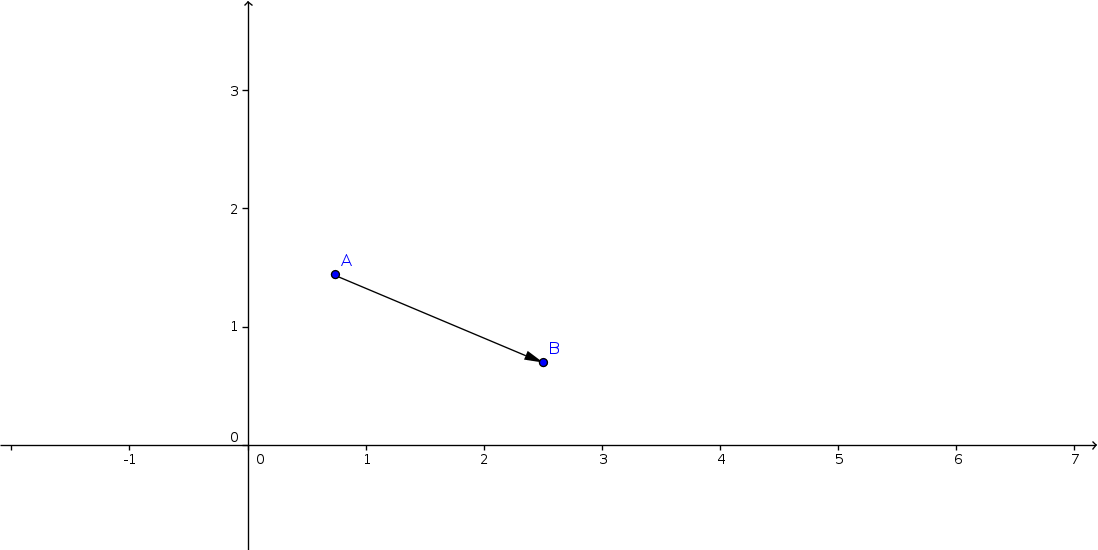
\includegraphics[width=15cm]{Graphics/wektor1}
\end{center}
\end{figure}

\section*{Własności}

Każdy wektor posiada następujące własności:
\begin{itemize}
    \item kierunek -- zgodny z kierunkiem prostej, na której leżą punkty $A$ i $B$,
    \item zwrot -- zaznaczony grotem wektora sposób uporządkowania punktów $A$ i $B$,
    \item punkt przyłożenia (zaczepienia) -- miejsce lokalizacji początku wektora.
\end{itemize}

Jeśli wektor $\overrightarrow{AB}$ umieścić w kartezjańskim układzie współrzędnych, w którym punkt $A$ ma współrzędne $(x_a,y_a)$, a punkt $B$ $(x_b,y_b)$, to liczby $a = x_b - x_a$ oraz $b = y_b - y_a$ nazywamy współrzędnymi (składowymi) wektora $\overrightarrow{AB}$, co zapisujemy w postaci $\overrightarrow{AB} = [a,b]$.

\section*{Powiązane definicje}

\paragraph{Długość wektora} wyraża się wzorem:
\[
    \left|\overrightarrow{AB}\right| = \sqrt{a^2 + b^2} = \sqrt{\left(x_b - x_a\right)^2 + \left(y_b - y_a\right)^2}
\]

\paragraph{Wektory równoległe} to dwa niezerowe wektory, które wyznaczają ten sam kierunek. Aby to łatwo sprawdzić, wystarczy policzyć \emph{iloczyn wektorowy}. Jeśli jest on równy 0, dwa wektory są równoległe.

\paragraph{Wektory przeciwne} to dwa wektory, posiadające tę samą długość i kierunek, lecz przeciwne zwroty. Dla wektora $\overrightarrow{v}$ wektorem przeciwnym jest $-\overrightarrow{v}$.

\paragraph{Wektor swobodny} to wektor, dla których nie określono punktu zaczepienia. Definiuje się je określając współrzędne.

\paragraph{Wektor zerowy} to wektor, którego początek i koniec pokrywają się. Nie posiada on kierunku oraz zwrotu, zatem jest równoległy do każdego innego wektora.

\paragraph{Wektory prostopadłe} to wektory, których wyznaczane kierunki są prostopadłe. Aby łatwo stwierdzić ten fakt, liczy się \emph{iloczyn skalarny}, który jest równy 0 wtedy i tylko wtedy, gdy wektory są prostopadłe.

\paragraph{Wektor jednostkowy (wersor)} to wektor o długości 1, posiadający kierunek i zwrot jednej z osi układu współrzędnych

\section*{Działania na wektorach}

\subsection*{Dodawanie}

Mając dwa wektory $\vect{a} = [x_a, y_a]$ oraz $\vect{b} = [x_b, y_b]$ (\emph{wektory składowe} -- uczestniczące w działaniu), dodawszy je, otrzymujemy nowy wektor $\vect{c} = \vect{a} = \vect{b} = [x_a + x_b, y_a + y_b]$. Jego współrzędne równe są sumie współrzędnych wektorów składowych. Suma wektorów zwana jest często \emph{wypadkową}.

Da się również obliczyć sumę wektorów geometrycznie. Aby dodać dwa wektory $\vect{AB}$ i $\vect{BC}$ zaczepiamy pierwszy wektor w punkcie $A$, drugi w końcu pierwszego wektora (punkcie $B$). Wektorem wypadkowym jest wektor biegnący od początku pierwszego wektora (punktu $A$) do końca ostatniego wektora (punktu $C$).

Dodawanie wektorów podlega prawu przemienności oraz łączności.

\paragraph{Przykład} Sumą wektorów $\vect{u} = [5,-3]$ i $\vect{v} = [2,7]$ jest wektor $\vect{u+v} = [5+2, -3+7] = [7,4]$.

\begin{figure}[h]
\begin{center}
    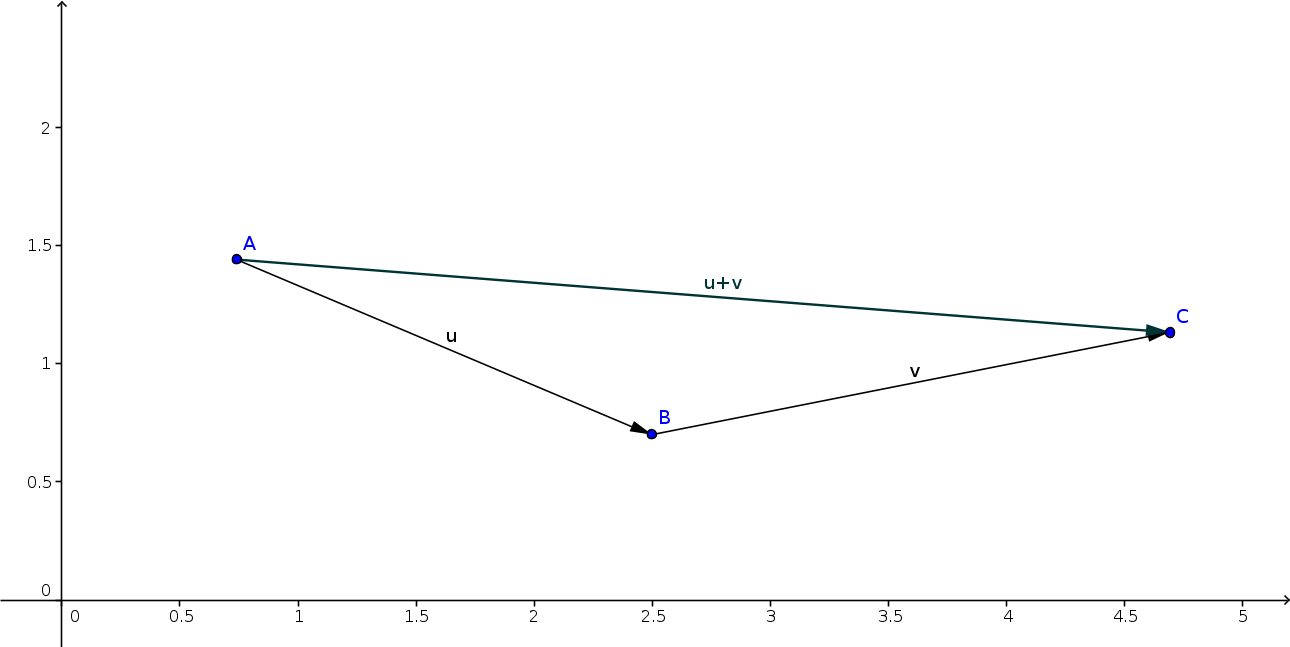
\includegraphics[width=15cm]{Graphics/wektor2}
\end{center}
\end{figure}

\subsection*{Odejmowanie wektorów}

Różnica wektorów to wektor, o współrzędnych równych różnicy współrzędnych wektorów składowych. Dla $\vect{a} = [x_a, y_a]$ oraz $\vect{b} = [x_b, y_b]$ wektor różnicy jest równy $\vect{a-b} = [x_a - x_b, y_a - y_b]$. A więc odjęcie wektora $\vect{b}$ od wektora $\vect{a}$ jest równoznaczne dodaniu do wektora $\vect{a}$ wektora $-\vect{b}$.

\subsection*{Mnożenie wektorów przez skalar}

Dla wektora $\vect{a} = [x_a, y_b]$ oraz liczby $k \in \mathbb{R}$ iloczyn równy jest $k\vect{a} = [k\cdot x_a, k\cdot y_a]$. 

Dla dowolnych liczb rzeczywistych $k$ i $l$ oraz wektorów $\vect u$ i $\vect v$ prawdziwe są twierdzenia:

\begin{itemize}
    \item $k\left(l\vect{u}\right) = (k\cdot l)\vect{u}$
    \item $k\left(\vect{u} + \vect{v}\right) = k\vect{u} + k\vect{v}$
    \item $(k+l)\vect{u} = k\vect{u} + l\vect{u}$
\end{itemize}

\subsection*{Iloczyn skalarny}

Dla wektorów $\vect a = [x_a, y_b]$ i $\vect b = [x_b, y_b]$ iloczynem skalarnym wektorów jest liczba:
\[
    \vect a \circ \vect b = \left| \vect a\right| \cdot \left| \vect b\right| \cdot \cos\angle
\left(\vect a, \vect b\right) = x_a \cdot x_b + y_a \cdot y_b
\]

\subsubsection*{Własności iloczynu skalarnego}

\begin{itemize}
    \item Przemienność:
    $$\vect u \circ \vect v = \vect v \circ \vect u$$
    \item Łączność mnożenia wektora z wektorem pomnożonym przez skalar:
    $$\left(k\vect u\right)\circ\vect v = \vect u \circ \left(k\vect v\right) = k\left(\vect u \circ \vect v\right)$$
    \item Rozdzielność mnożenia względem dodawania wektorów:
    \[
        \vect a \circ \left( \vect b + \vect c\right) = \vect a \circ \vect b + \vect a \circ \vect c
    \]
    \item Iloczyn skalarny dwóch niezerowych prostopadłych wektorów jest równy 0.
    \[
        \vect u \circ \vect v = 0 \Rightarrow \vect u \perp \vect v
    \]

\paragraph{Przykład} Dla wektorów $\vect u = [3,5]$, $\vect v = [-5,2]$ iloczyn wynosi $\vect u \circ \vect v = 3\cdot(-5) + 5\cdot 2 = -8$.
\end{itemize}

\subsection*{Iloczyn wektorowy}

Dla dwóch niezerowych wektorów $\vect a = [x_a, y_a, z_a]$ i $\vect b = [x_b, y_b, z_b]$ iloczyn wektorowy jest równy:
\[
    \vect a \times \vect b = [y_a\cdot z_b - z_a\cdot y_b, z_a\cdot x_b - x_a\cdot z_b, x_a\cdot y_b - y_a\cdot x_b]
\]
Długość takiego iloczynu równa jest:
\[
    \left| \vect a \times \vect b \right| = \left|\vect a\right| \cdot \left|\vect b\right| \cdot \sin\angle\left(\vect a, \vect b\right)
\]
\subsubsection*{Własności iloczynu wektorowego}
\begin{itemize}
    \item $\vect u \times \vect v = -\vect v \times \vect u$
    \item $k\left(\vect u \times \vect v\right) = \left(k\vect u\right) \times \vect v$
    \item $\vect a \times \left(\vect b +\vect c\right) = \vect a \times \vect b + \vect a \times \vect c$
    \item $\vect u \times \vect v = 0 \Leftrightarrow \vect u \perp \vect v$
\end{itemize}

\paragraph{Długość iloczynu wektorowego} jest geometrycznie równa polu równoległoboku ułożonego z wektorów.

\begin{figure}[h]
\begin{center}
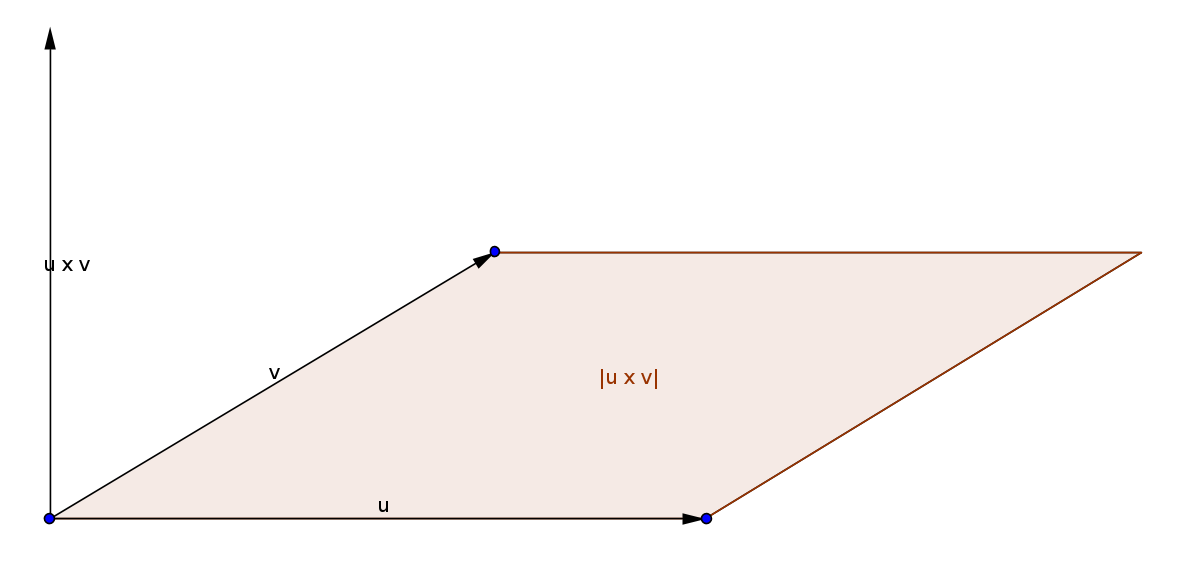
\includegraphics[width=15cm]{Graphics/wektor3}
\end{center}
\end{figure}

\end{document}
